\subsection{Risk management}
This section details what risks were identified in the beginning of the project and the potential impact they could have on reaching the main goal of this project. Next to the risks, mitigations are also defined. In the end, the risks are put into relation in a risk matrix. This helped in deciding which risks can be neglected and which ones must be mitigated at the very start of the project. 
\subsubsection{The Risks}
\begin{landscape}
	\rowcolors{2}{gray!25}{white}
	\begin{longtable}[H]
		{l|p{0.22\textwidth}| p{0.22\textwidth} | p{0.1\textwidth} | p{0.1\textwidth} | p{0.25\textwidth} | p{0.25\textwidth}}
		
		\textbf{Nr} & \textbf{Title} & \textbf{Description} & 
		\textbf{Max Harm [h]} & \textbf{Proba- bility} & \textbf{Prevention} &  
		\textbf{Behavior at entry}\\ \hline
		
		R1 & Underestimation of workload & One or more team members can't finish a feature in time or loses to much time on a minor feature & 70 & 25\% & Weekly scrum meetings with feedback about the current work progress. Estimate workload together. Include time reserve & Help each other, if one is struggling. Feature reduction as last resort. \\ 
		
		R2 & Work flow is not working & Tool chain is not working as planed. The used components aren't ideal for the problem & 30 & 15\% & Use experience to get a good setup and test it a lot in the beginning & Redefine tool chain or change single tool \\ 
		
		R3 & Communication problems & Team is not working together and each member is developing individually. Creation of incompatible interfaces. Talking with the industrial partner isn't possible as expected, due to time difference or not enough time & 70 & 20\% & Weekly scrum meetings and agreements. Already worked in other projects as a team before & Increase written documentation and working closer together. Having a fixed meeting with the industrial partner \\ 
		
		R4 & Lack of knowledge & Team has to little knowledge about Dafny, Visual Studio Code and the development of a Visual Studio Code Plugin & 80 & 10\% & Already experience with typescript for plugin development, as preparatory work informed about Dafny & Find necessary knowledge online, get help from Microsoft Research \\ 
		
		R5 & Data loss or manipulation & Data loss because of a server crash or open permissions to access and modify data & 20 & 3\% & Regularly backups and restrictive permissions to change files & Use backup to restore data. Extend safety measures \\ 
		
		R6 & Failure developer machine & One of the developer machines isn't working anymore. & 10 & 1\% & Limited, regularly commits and backups. & Switch temporary to the school computer and install the necessary tools. \\
		
		R7 & Implementing the DSL is too complicated or too difficult to use & The DSL would be needed to suggest possible contracts or to customize the best practices. & 100 & 30\% & This core feature has to be researched carefully so that it really fits our needs and that other developers can really use the plugin. & Read about DSL, talking to people which have already worked with it. \\
		
		R8 & Supporting all features on the different environments is not possible & Due to that Windows, OSX and Linux are quite different, it could be that some features aren't possible to implement on a platform or causes a big overhead to get it running & 10 & 25\% & Using as much of the standard API as possible. Implement specific features platform dependent & Disable a certain feature on a platform or look for a workaround. \\	
		
		R9 & Automatic installer of Dafny is not possible & Maybe because of security restrictions, it could be possible that you can't download and install additional software and set environment variables. & 35 & 20\% & Test if downloading of software can done inside VS Code. & Automatic installer can't be done inside the plugin. Switch to a different strategy and implement an automatic installer over a additional executable, which could also install the plugin in Visual Studio Code. \\
		
		R10 & Dafny and the way it is used is not well understood & If it is not clear how exactly the work flow of a Dafny programmer could be enhanced, there is the possibility that a lot of features could be implemented that don't better the programmer experience at all. & 80 & 20\% & Regular feedback loop with people that use Dafny. & Learn a lot about Dafny ourselves, talk to people that use Dafny.  \\
		
		\caption{Risk management}
		\label{tab:Risk management}
	\end{longtable}
\end{landscape}

\subsubsection{Risk Matrix}
\begin{figure}[H]
	\centering
	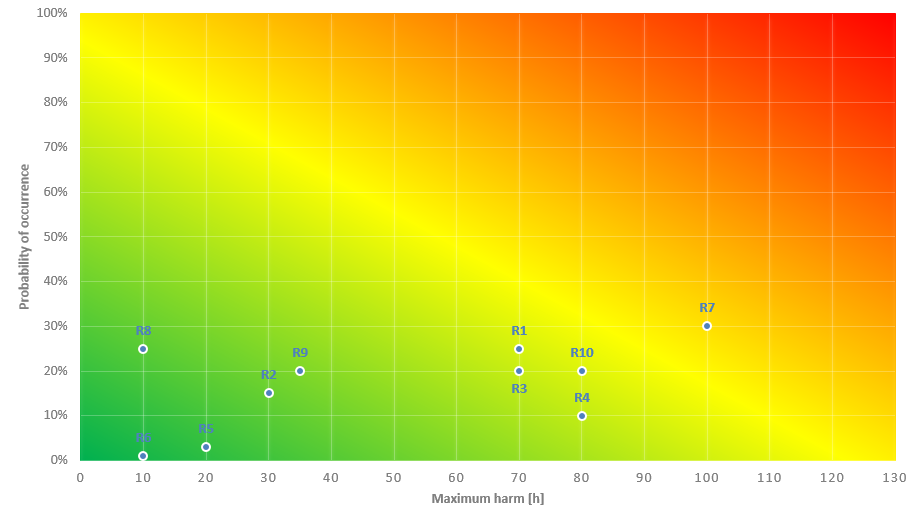
\includegraphics[width=1\textwidth]{img/riskmatrix}
	\caption{Risk Matrix}
	\label{fig:Risk Maxtrix}
\end{figure}